用于并行编程的共享内存模型的优点是提供单一、共享的内存。我们不需要显式的从并行任务中访问内存(除了适当的同步以避免数据竞争)。当某些类型的加速器设备(例如集成GPU)与主机CPU共享内存时,许多独立加速器有自己的内存,不与CPU的内存在一起,如图3-1所示。\par

\hspace*{\fill} \par %插入空行
图3-1 多个独立的内存
\begin{center}
	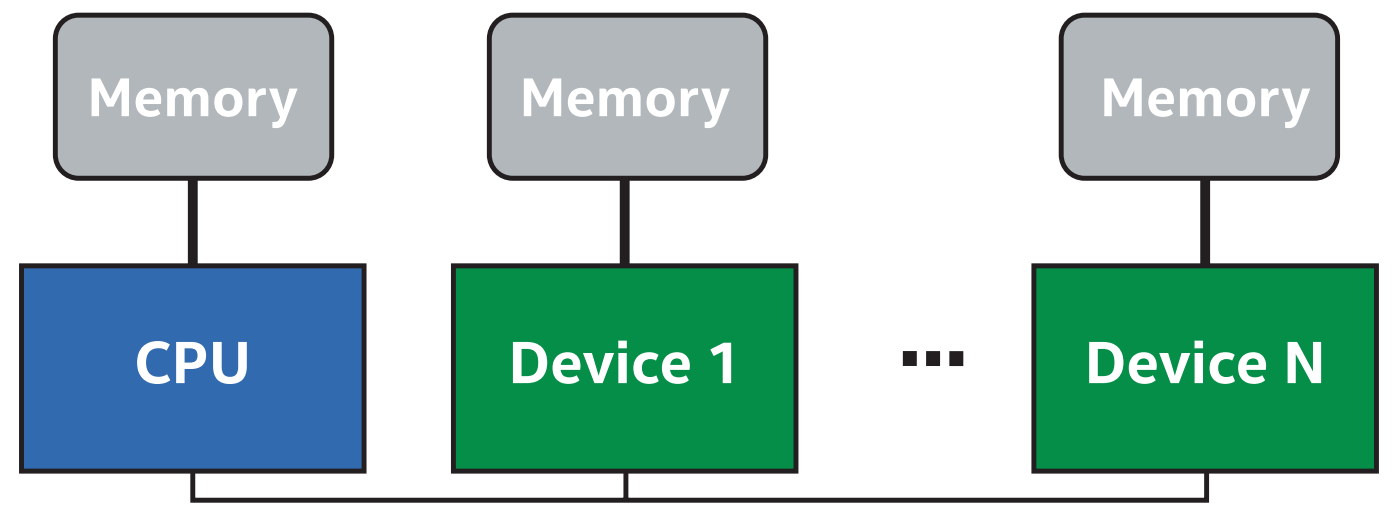
\includegraphics[width=0.8\textwidth]{content/chapter-3/images/2}
\end{center}









